\begin{frame}[fragile]{Branching: Fetch Remote Branches}
  \begin{columns}
    \begin{column}{0.7\textwidth}
      \begin{figure}
        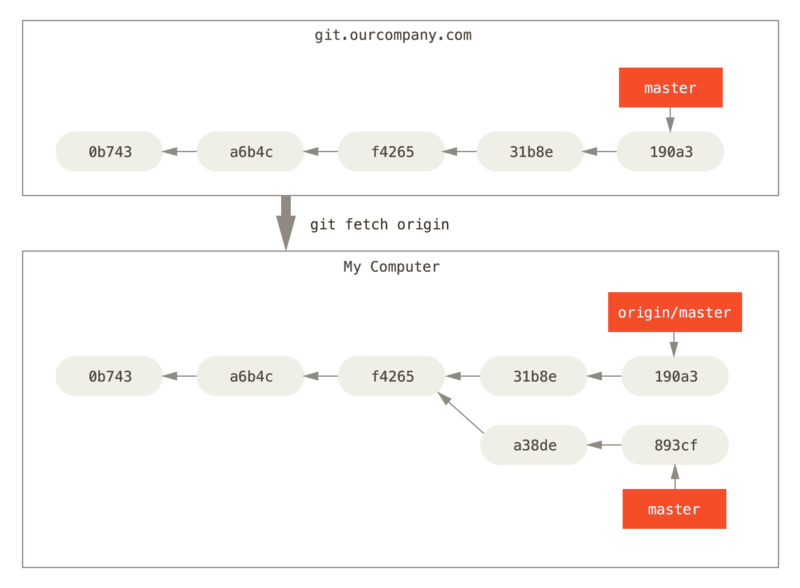
\includegraphics[width=0.9\textwidth]{branching/remote-branches-3}
        \caption{Updates remote-tracking branches}
      \end{figure}
    \end{column}
    \begin{column}{0.3\textwidth}
      \begin{flushleft}
        1. Fetch any data that you don’t yet have from remote
      \end{flushleft}
      \begin{flushleft}
        2. Update the local version database (the Git directory)
      \end{flushleft}
      \begin{flushleft}
        3. Move the `origin/master` pointer to the new commit
      \end{flushleft}
    \end{column}
  \end{columns}
\end{frame}
